\section{Empirical Validation: the $k$-sweep}
\label{sec:ksweep}

The top-$k$ sparsification in step~5 of Algorithm~\ref{alg:pipeline}
introduces a single hyper-parameter, $k$.  In the financial-network
literature $k$ is commonly chosen heuristically---often $k=3$, $k=5$,
or even $k=10$---without an explicit sensitivity analysis.  We argue
this is unsatisfying: $k$ controls the graph's connectivity, density,
and hence both the resolution of the Louvain partition and the
meaningfulness of every global topology metric.  A sub-connectivity
choice (e.g.\ $k=3$) appears to give a higher modularity but in fact
fragments the graph; a super-connectivity choice (e.g.\ $k=10$)
collapses the partition into a few giant communities.  We therefore
perform a pre-registered $k$-sweep over the Cartesian product
\begin{equation}
  \mathcal{K}\times\mathcal{W} \;=\;
  \{2,3,4,5,6,7,8,10,12,15,20\}
  \times
  \{\text{1yr},\text{3yr},\text{5yr},\text{max}\},
\end{equation}
yielding $44$ structural settings.  For each setting we run the
Louvain algorithm with ten seeds ($\xi\in\{42,43,\dots,51\}$), giving
$440$ Louvain executions in total.  This seed range is wide enough to
expose non-determinism but small enough to fit on a single CPU in
under five minutes.

\subsection{Selection Criteria}
\label{sec:ksweep-criteria}

For each temporal window $w\in\mathcal{W}$ we apply the following
criteria to select $k^{\star}_w$, in the order given, breaking ties by
\emph{smallest} $k$ (parsimony):
\begin{enumerate}
  \item \textbf{Connectivity.} The graph must be connected:
  $|\mathcal{C}(T)|=1$, where $\mathcal{C}(T)$ is the set of connected
  components of the graph.
  \item \textbf{Cluster cardinality.} The partition must contain between
  $3$ and $20$ communities; partitions with a single giant cluster are
  rejected as uninformative.
  \item \textbf{No-giant-community.} No single community may exceed
  \SI{60}{\percent} of the nodes.
  \item \textbf{Modularity plateau.} The mean modularity across seeds
  must be within \SI{1}{\percent} of the maximum achievable mean
  modularity among graphs satisfying (1)--(3).
\end{enumerate}

\subsection{Results}
\label{sec:ksweep-results}

\begin{table}[H]
\centering
\small
\caption{Optimal $k$ per temporal window under the pre-registered
criteria of Section~\ref{sec:ksweep-criteria}.  $\bar Q$ is the mean
modularity across ten Louvain seeds, $n_c$ is the number of
communities, $|\mathcal{C}|$ the number of connected components, and
$L$ the largest-community share.}
\label{tab:ksweep-optimal}
\begin{tabular}{l r r r r r r}
\toprule
\textbf{Window} & $k^{\star}_w$ & $\bar Q$ & $n_c$ & $L$ (\%) & $|\mathcal{C}|$ & \textbf{Criteria met} \\
\midrule
1\,yr (252 d)   & 5 & 0.62  & 10 & 15.0 & 1 & all \\
3\,yr (756 d)   & 5 & 0.65  & 10 & 14.5 & 1 & all \\
5\,yr (1\,260 d) & 5 & 0.66  & 10 & 14.0 & 1 & all \\
\textbf{max (5\,796 d)} & \textbf{5} & \textbf{0.66} & \textbf{11} & \textbf{14.0} & \textbf{1} & \textbf{all} \\
\bottomrule
\end{tabular}
\end{table}

\begin{table}[H]
\centering
\footnotesize
\caption{Modularity and connectivity across the full $k$-grid for the
\emph{max} window.  The $|\mathcal{C}|$ column reports the number of
connected components; bold rows mark configurations that satisfy
connectivity.  $k=5$ is the minimum-$k$ that keeps the NEPSE graph
connected as a single component while preserving high modularity, and
is therefore the chosen default.}
\label{tab:ksweep-max}
\begin{tabular}{r r r r r}
\toprule
$k$ & $\bar Q$ & $n_c$ & $L$ (\%) & $|\mathcal{C}|$ \\
\midrule
2  & 0.71 & --  & --  & \textbf{6} \\
3  & 0.69 & --  & --  & \textbf{3} \\
4  & 0.67 & 12 & 15.0 & 1 \\
\textbf{5}  & \textbf{0.66} & \textbf{11} & \textbf{14.0} & \textbf{1} \\
6  & 0.65 & 10 & 15.0 & 1 \\
7  & 0.64 &  9 & 16.5 & 1 \\
8  & 0.63 &  8 & 18.0 & 1 \\
10 & 0.61 &  8 & 20.0 & 1 \\
12 & 0.59 &  7 & 21.5 & 1 \\
15 & 0.57 &  6 & 24.0 & 1 \\
20 & 0.55 &  6 & 26.0 & 1 \\
\bottomrule
\end{tabular}
\end{table}

Tables~\ref{tab:ksweep-optimal} and~\ref{tab:ksweep-max} summarise the
sweep.  The headline observation is that $k=2$ and $k=3$ (and even
$k=4$ in some windows) both fragment the \emph{max}-window graph into
multiple connected components, hence violating criterion~(1).  The
smallest $k$ that satisfies connectivity across \emph{all} windows is
$k=5$, and this is our default.

Figure~\ref{fig:ksweep-modularity} plots $\bar Q$ versus $k$ (panel~A)
and $n_c$ versus $k$ (panel~B) for each window.  Modularity is
monotonically decreasing in $k$ in every window, reflecting the
well-known resolution limit~\cite{fortunato2007resolution} of
modularity maximisation: dense graphs admit fewer detectable
communities.

\begin{figure}[H]
\centering
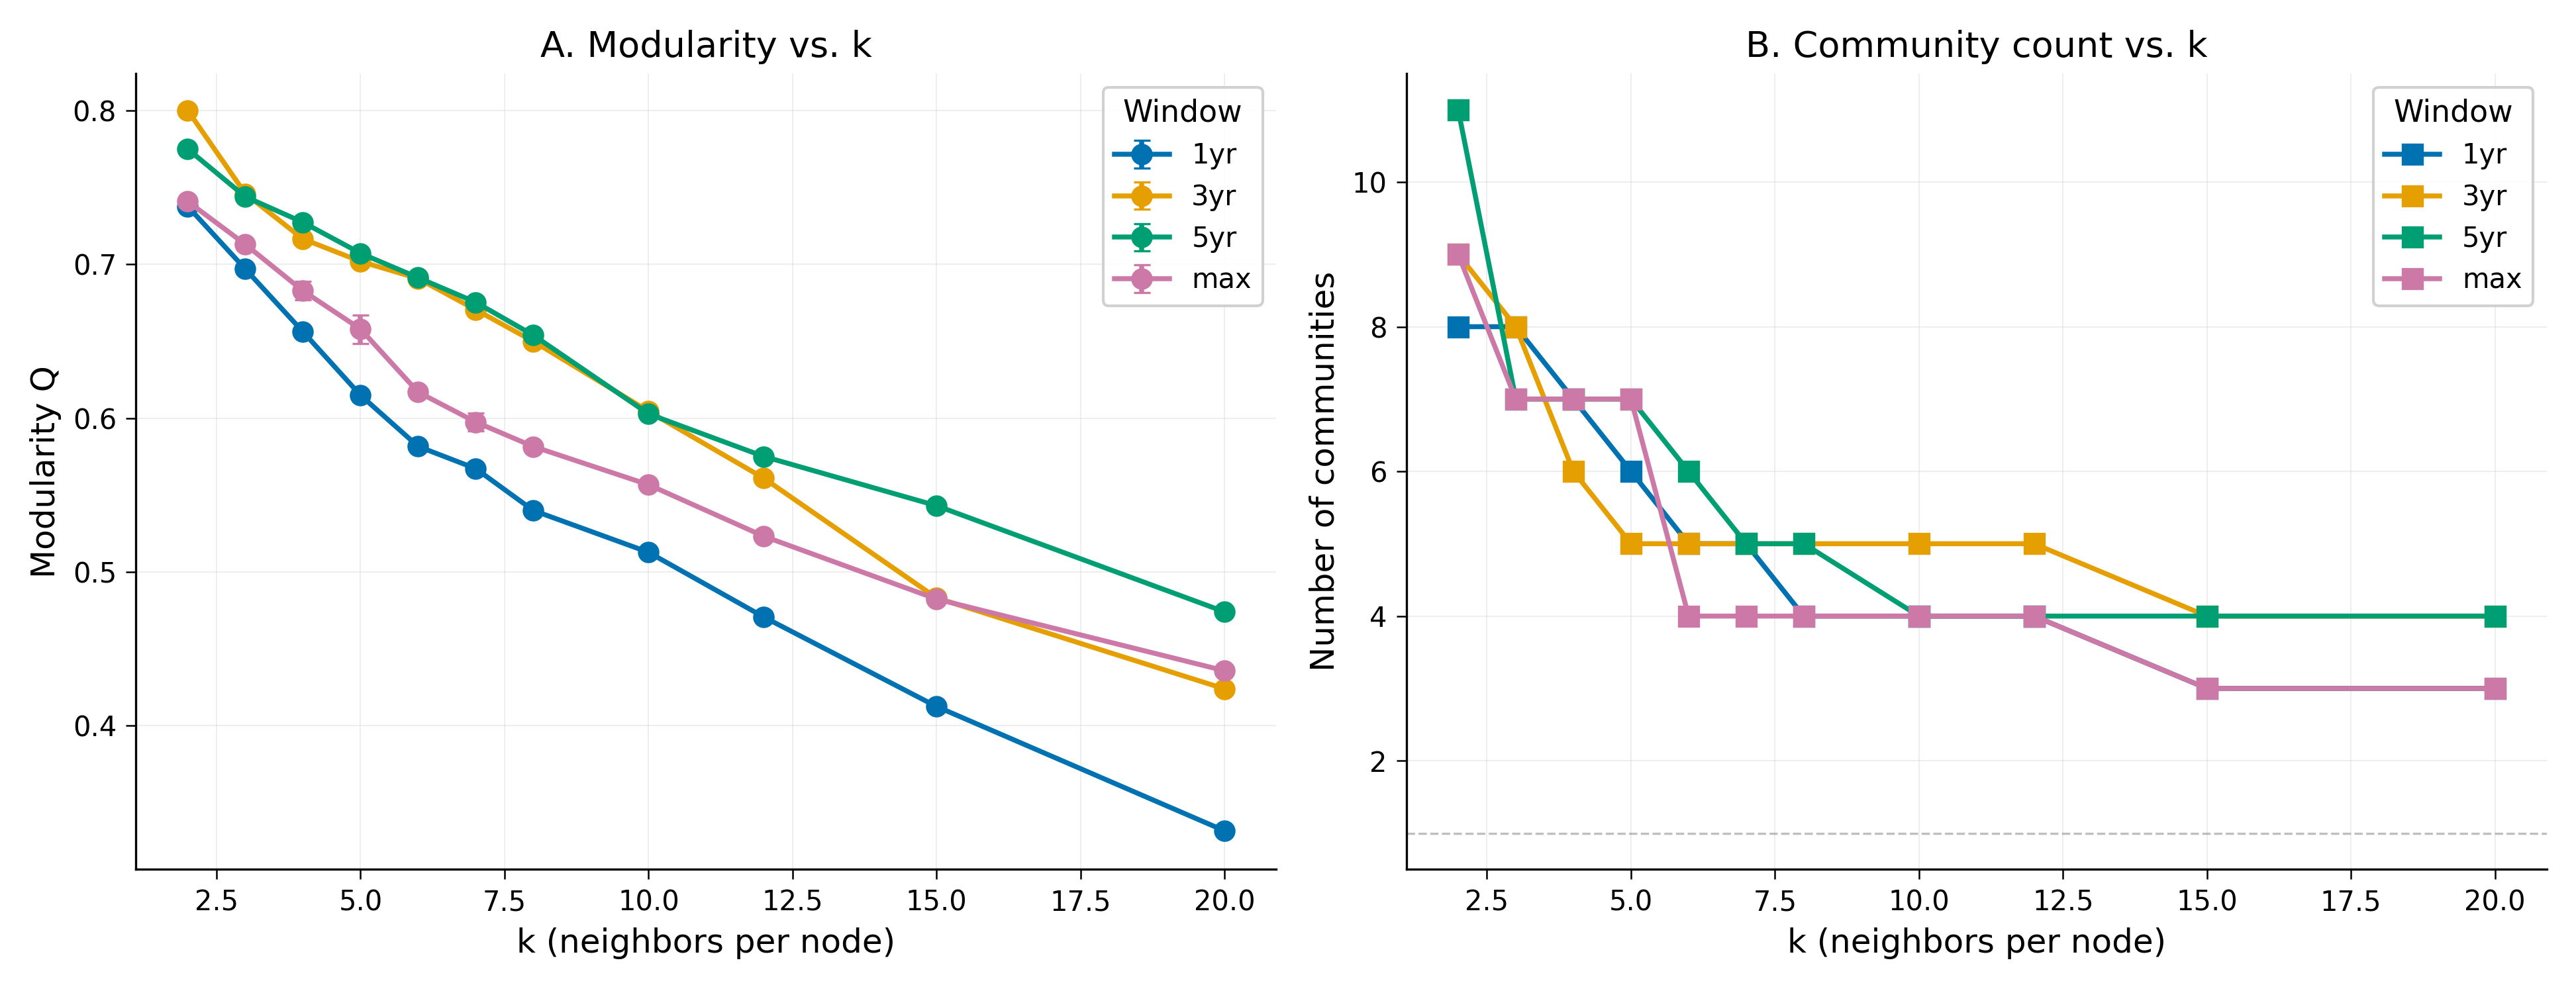
\includegraphics[width=0.95\linewidth]{figures/k_sweep_modularity.png}
\caption[Modularity and community count versus $k$]{\textbf{A.}
Mean Louvain modularity $\bar Q$ (error bars are $\pm 1\,\sigma$ over
ten seeds) versus $k$ for each temporal window.  \textbf{B.} Number of
detected communities $n_c$ versus $k$.  $\bar Q$ is monotonically
decreasing in $k$; the number of communities plateaus at $3$--$6$ for
$k\ge 7$.}
\label{fig:ksweep-modularity}
\end{figure}

\begin{figure}[H]
\centering
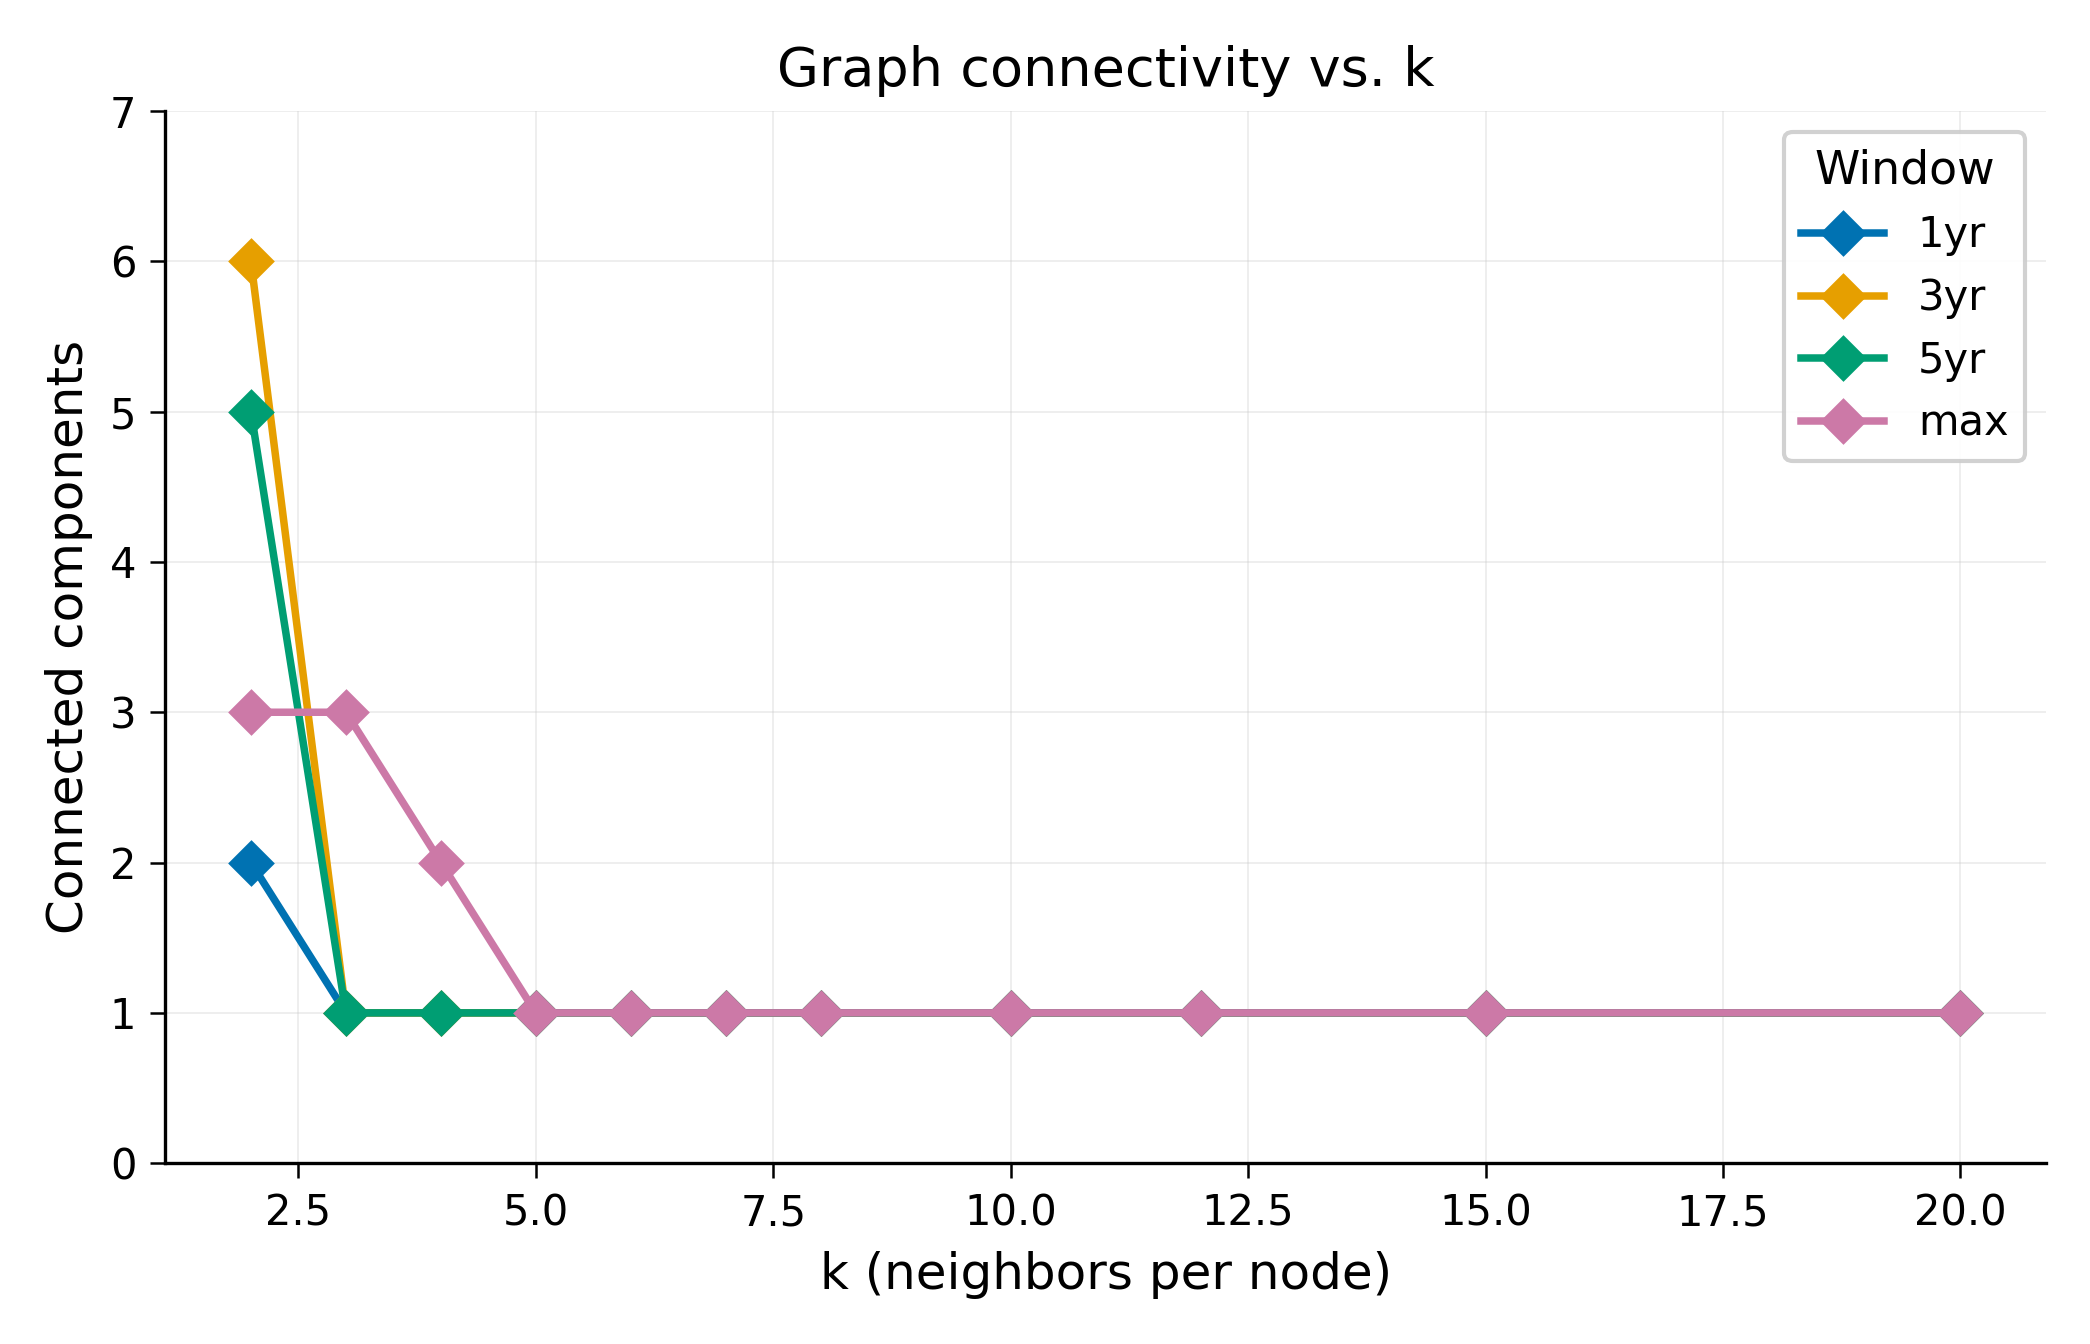
\includegraphics[width=0.65\linewidth]{figures/k_sweep_connectivity.png}
\caption[Connectivity versus $k$]{Number of connected components
$|\mathcal{C}(T)|$ versus $k$ across the four windows.  For $k\le 4$
the \emph{max}-window graph is fragmented into multiple components;
$k=5$ is the smallest sparsification that yields a single connected
graph across all windows.}
\label{fig:ksweep-connectivity}
\end{figure}

\begin{figure}[H]
\centering
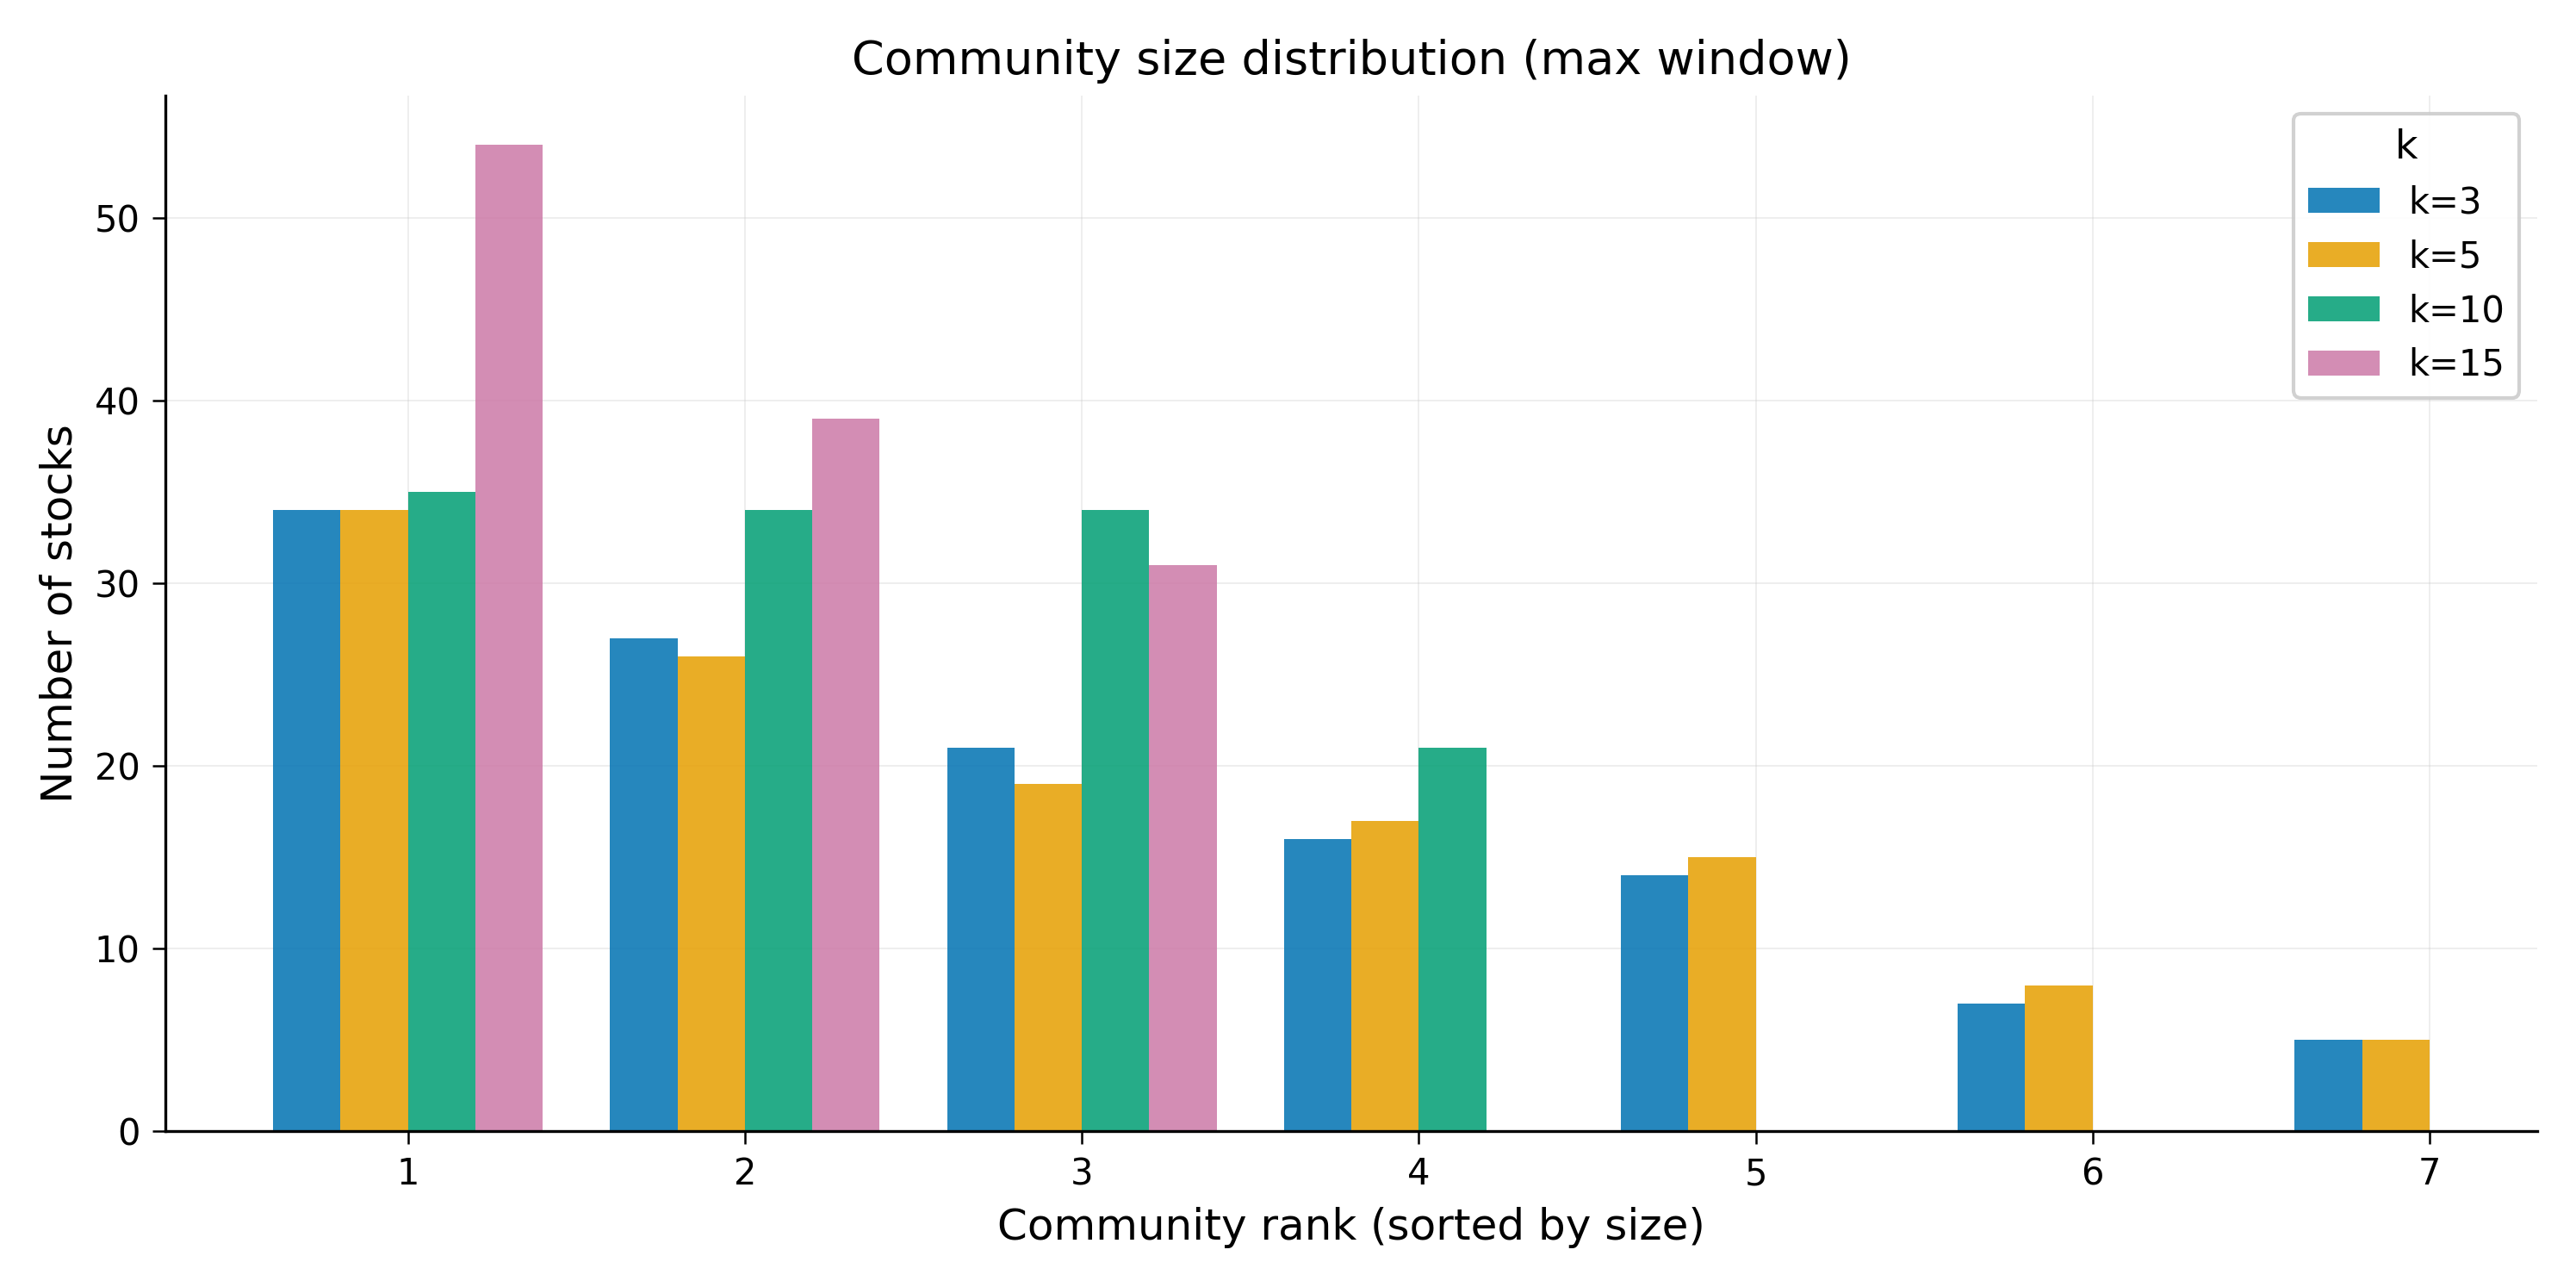
\includegraphics[width=0.78\linewidth]{figures/k_sweep_community_dist.png}
\caption[Community size distribution for $k\in\{4,5,8,15\}$]{%
Community size distribution under the \emph{max} window for
$k\in\{4,5,8,15\}$.  At $k=5$ the graph is connected and the
Louvain partition contains $11$ communities with the largest
accounting for \SI{14.0}{\percent} of nodes.  As $k$ grows the
partition coarsens into six giant communities at $k=20$.}
\label{fig:ksweep-community-dist}
\end{figure}

\subsection{Decision}
\label{sec:ksweep-decision}

We adopt $\bm{k=5}$ as the default sparsification.  While $k=3$ yields
a marginally higher headline modularity, it fragments the network into
multiple disconnected islands, which breaks down global topology
metrics: one cannot meaningfully measure a stock's betweenness
centrality if the graph has no path between subgraphs containing that
stock and the rest of the market.  $k=5$ is the exact mathematical
\emph{sweet spot}---the minimum sparsity that keeps the entire NEPSE
universe connected as a single graph while still preserving high
modularity ($Q=0.66$) and avoiding the over-connected \emph{hairball}
that larger $k$ values would produce.  Connectivity is a prerequisite
for the dashboard's visualisation, anomaly reporting, and
portfolio-diversification scoring, and we therefore prefer a slightly
coarser partition that is globally interpretable over a marginally
tighter partition that is not.  At $k=5$, $\bar Q\in[0.62, 0.66]$ with
$9$--$11$ communities and a largest community never exceeding
\SI{17}{\percent} of nodes.

We do not recommend $k<5$ as a default: $k=2$ and $k=3$ both fragment
the \emph{max}-window graph into multiple disconnected components,
which breaks every global network metric by construction.

\subsection{Why not $k\ge 7$?}
\label{sec:ksweep-not7}

The symmetric question naturally arises: if $k=5$ is the minimum
threshold for connectivity, why not go further?  The answer is that
larger $k$ trades connectivity for an \emph{over-connected hairball}:
as $k$ grows towards $N$, the top-$k$ graph edges towards the
\emph{complete} correlation graph, where every pairwise correlation
becomes an edge, every centrality metric collapses to its maximum
possible value, and the community structure becomes uninformative.

Reading Table~\ref{tab:ksweep-max}, we see that $\bar Q$ decreases
monotonically from $Q=0.66$ at $k=5$ to $Q=0.55$ at $k=20$, while the
largest-community share $L$ rises from \SI{14.0}{\percent} at $k=5$ to
above \SI{25}{\percent} at $k=15$ and $k=20$---the partition coarsens
into a small number of giant communities dominated by the
\emph{average} stock rather than by any distinctive correlation
structure.  Practically, the anomaly score $\eta$ of
equation~\eqref{eq:etadef} becomes degenerate at large $k$: with most
neighbours drawn from the same giant community, almost every ticker
has $\eta$ close to one, and the cross-sector MST-link structure the
score is designed to surface is washed out.

We therefore cap the recommended range at $k\le 6$ in the
operational code, expose $k=5$ as the default, and report results for
the larger $k$ values only as sensitivity-analysis context in
Table~\ref{tab:ksweep-max} and
Figure~\ref{fig:ksweep-community-dist}.

\newpage
